\chapter{Software Requirements Specification}
\label{ch:srs}
This chapter will contain the functional and non-functional requirements of the project.
\section{List of functions}
List of key features for the "Improving Medical Education through Immersive Virtual Reality (MetaMed)" project:\\
\textbf{Realistic medical simulations:}\\ Create highly realistic medical scenarios and procedures that faithfully mimic real medical experiences, including various medical specialties.\\
\textbf{Haptic feedback integration:}\\ Integrate tactile feedback devices to provide tactile sensations, increasing the realism of medical training and allowing students to develop their tactile skills.\\
\textbf{Immersive 3D Environments:}\\ Create immersive, 3D virtual environments that accurately represent medical settings, including operating rooms, medical instruments, and anatomical structures.\\
\textbf{Interactivity:}\\Enables hands-on interaction with virtual medical tools, instruments, and equipment, allowing students to perform medical tasks and procedures.\\
\textbf{Remote Access:}\\ Enable medical students to access a metaverse-based medical training platform from remote locations, facilitating flexible learning.
\section{Test plan (test level, test techniques)}
\text{Test plan for our project will be as:}
\begin{itemize}
    \item Movement in VR 
    \item Interaction with Objects
    \item Treatement to Patient
\end{itemize}
\section{Use Case Diagram}
Here is the Use Case Diagram of the Project.
\begin{figure}[h]
    \centering
    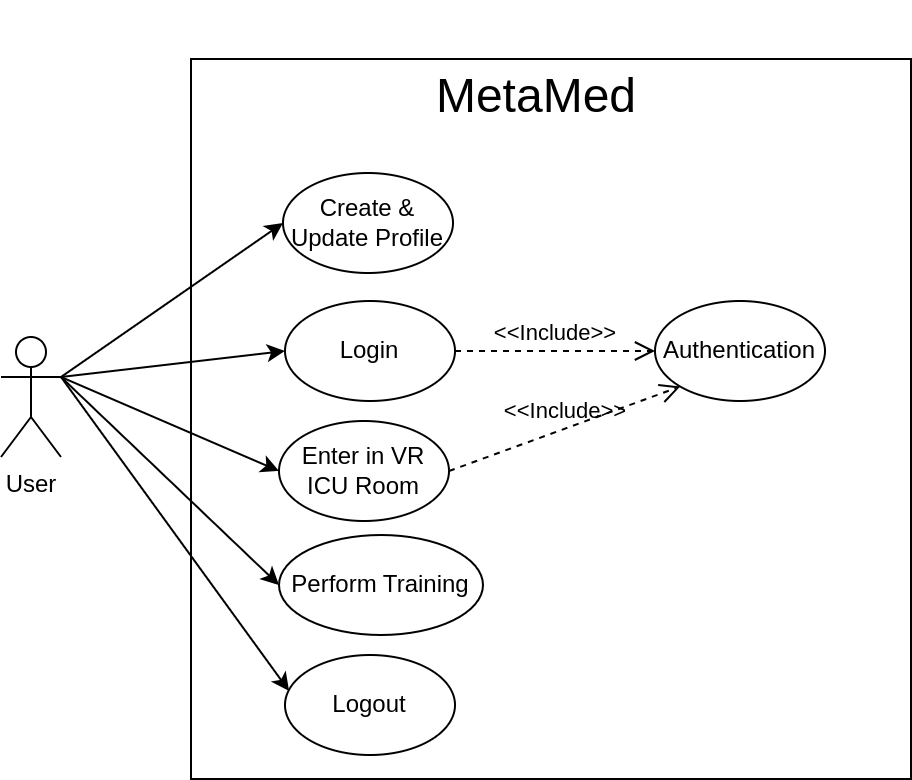
\includegraphics[width=0.6\textwidth, height=0.3\textheight]{Images/Use Case.drawio.png}
    \caption{Use Case Diagram}
    \label{fig:system-diagram}
\end{figure}

\section{Software Development Plan}
\text{Software Development Plan for our project will be as:}
\begin{itemize}
    \item Project Overview 
    \item Requirements Gathering and Analysis
    \item System Design
    \item Development
    \item Testing
    \item Documentation
    \item Management
\end{itemize}

\section{System Diagram}
It is the System Diagram of the Project.
\begin{figure}[h]
    \centering
    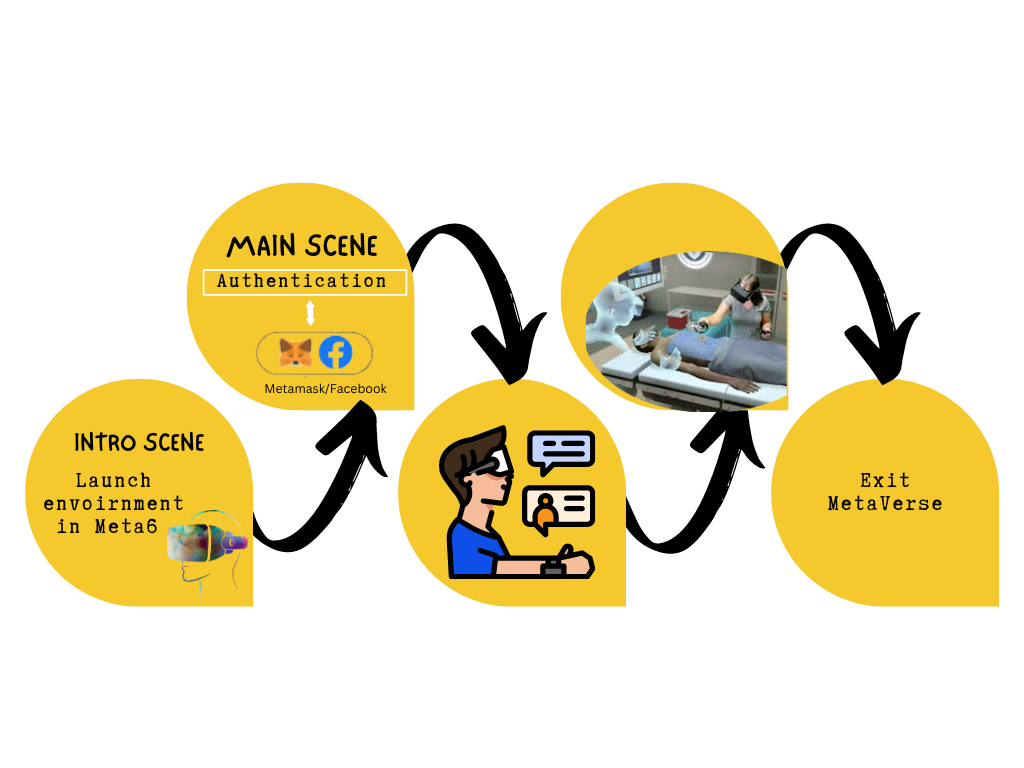
\includegraphics[width=1\linewidth, height=0.65\linewidth]{Images/system.png}
    \caption{System Diagram}
\end{figure}
\newpage
\section{Activity Daigram}
The activity diagram aims to illustrate the entire process of project working and demonstration.
\begin{figure}[h]
    \centering
    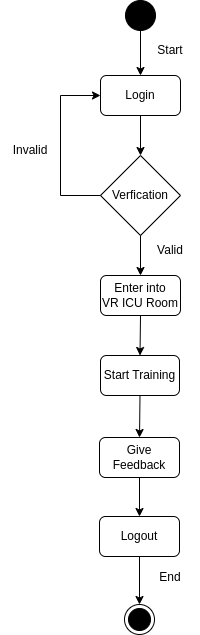
\includegraphics[width=0.25\linewidth]{Images/Activity.drawio.png}
    \caption{Activity Diagram}
\end{figure}
\newpage
\section{Tools and Technologies used}
\subsection{C-Sharp:}
C-Sharp is a programming language developed by Microsoft that runs on the .NET Framework. C-Sharp is used to develop web apps, desktop apps, mobile apps, games and much more.
\begin{figure}[h]
	\centering
	
\includegraphics[width=0.1\linewidth, height=0.1\linewidth]{Images/CSharp.png}
	\caption{C-Sharp\cite{csharp}}
\end{figure}
\subsection{Blender}
Blender is a free, open-source 3D graphics software used for creating animated films, visual effects, art, models, motion graphics, interactive applications, and virtual reality.
\begin{figure}[h]
	\centering
	
\includegraphics[width=0.2\linewidth, height=0.2\linewidth]{Images/blender.png}
	\caption{blender\cite{blender}}
\end{figure}
\subsection{Git}
Git is a distributed version control system that tracks versions of files. It is used to control source code and collaboratively developing software.
\begin{figure}[h]
	\centering
	
\includegraphics[width=0.2\linewidth, height=0.2\linewidth]{Images/git.png}
	\caption{git\cite{git-logo}}
\end{figure}
\subsection{GitHub}
GitHub is a platform for developers to create, store, manage, and share their code, with Git software providing distributed version control, access control, task management, and continuous integration.
\begin{figure}[h]
	\centering
	
\includegraphics[width=0.1\linewidth, height=0.1\linewidth]{Images/GitHub.png}
	\caption{GitHub\cite{github-logo}}
\end{figure}
\subsection{Meta}
Meta-verse is a sophisticated, interconnected virtual world that enhances user experiences by creating seamless, immersive digital environments.
\begin{figure}[h]
	\centering
	
\includegraphics[width=0.2\linewidth, height=0.2\linewidth]{Images/meta.png}
	\caption{Meta\cite{meta}}
\end{figure}
\subsection{Unity}
Unity was utilized to develop 3D and 2D games, interactive simulations, and has been widely adopted by various industries beyond video gaming.
\begin{figure}[h]
	\centering
	
\includegraphics[width=0.2\linewidth,height=0.2\linewidth]{Images/unity.png}
	\caption{Unity\cite{Unity}}
\end{figure}
\newpage
\subsection{Meta Quest 2}
Project MetaMed VR utilized Meta Quest 2 for its advanced features like hand tracking and gesture recognition, enhancing medical education through immersive virtual reality experiences.
\begin{figure}[h]
	\centering
	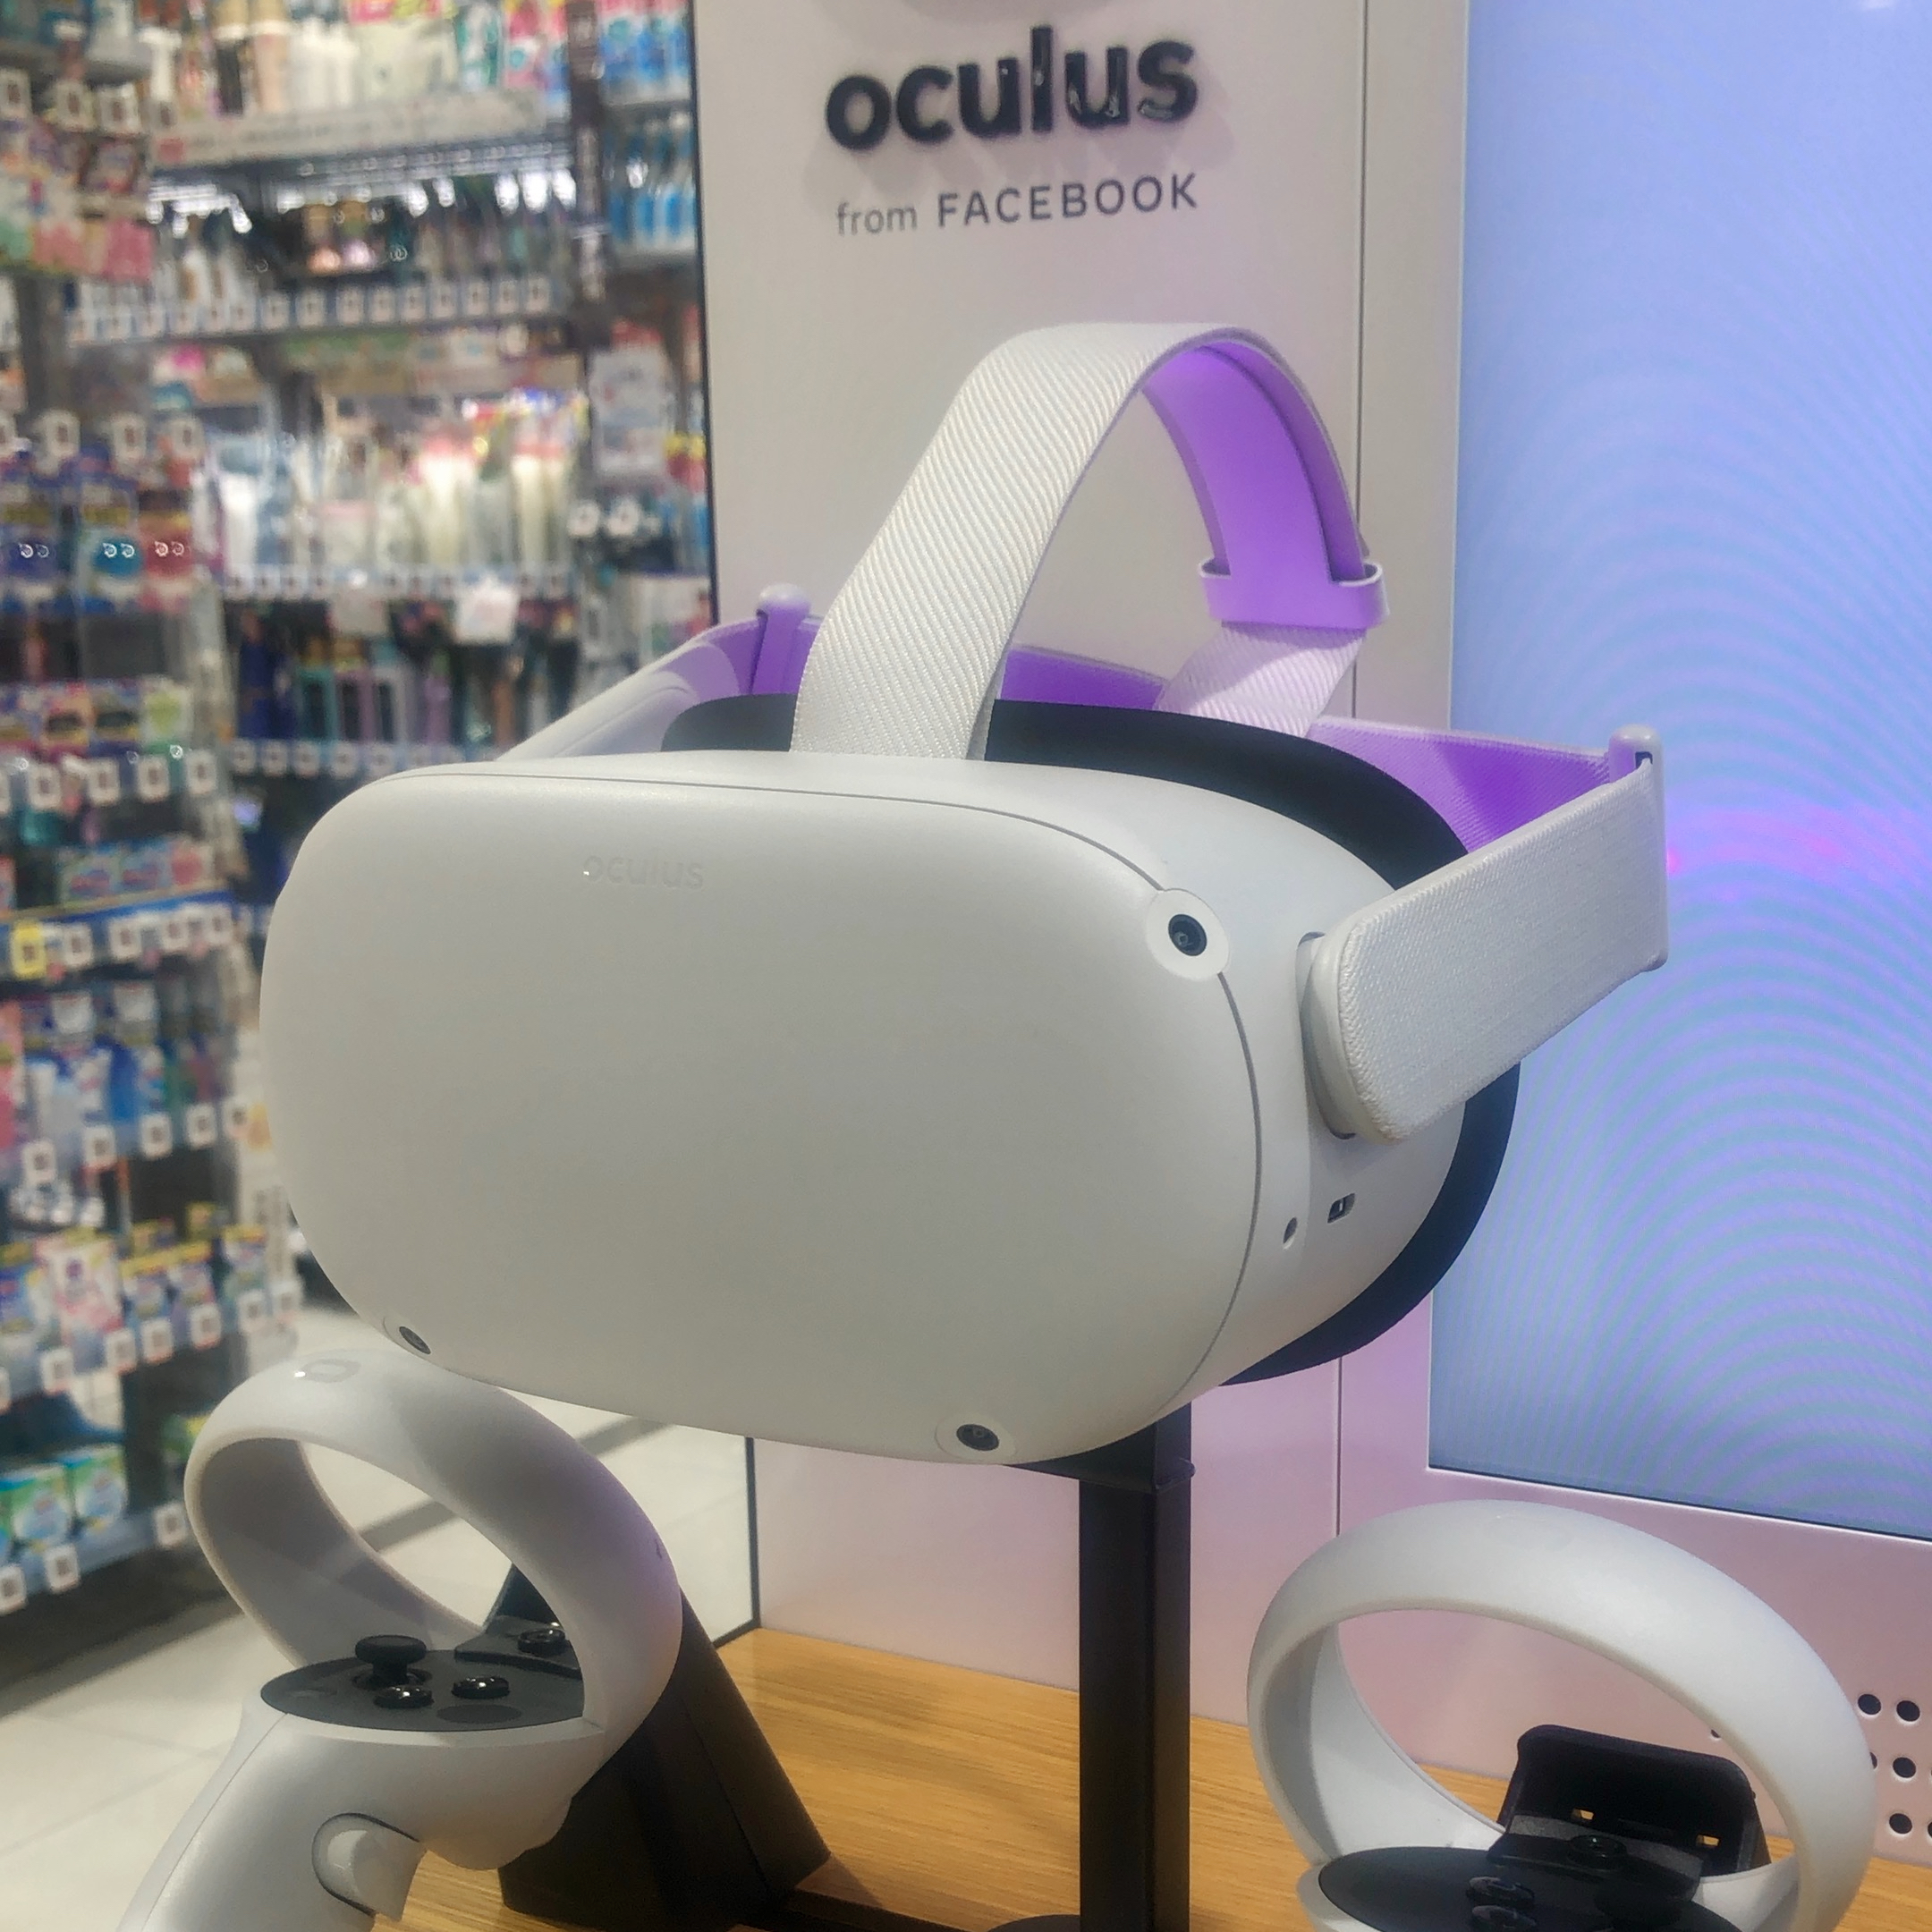
\includegraphics[width=0.4\linewidth,height=0.3\linewidth]{Images/metaquest2.png}
	\caption{Meta Quest 2\cite{metaquest}}
\end{figure}
\subsection{Microsoft Visual C++}
Microsoft Visual C++ is integrated with Unity 3D to optimize code, improve performance, and manage memory in complex applications, ensuring smooth and efficient gameplay.
\begin{figure}[h]
	\centering
	
\includegraphics[width=0.2\linewidth,height=0.2\linewidth]{Images/VS Code.png}
	\caption{Microsoft Visual C++\cite{visual-studio-icon}}
\end{figure}